% 64-24(64쪽) — 반지름 16, 중심각 θ 인 부채꼴 모양의 종이(왼쪽)를 말아 밑면의 반지름이 r 인 원뿔(오른쪽)을 만드는 그림.
% 스캔 화질이 낮아 TikZ 로 다시 그림 — 라벨은 원문 그대로(θ·16·r)만 두고 θ 의 값을 읽을 수 있는 눈금은 넣지 않는다.
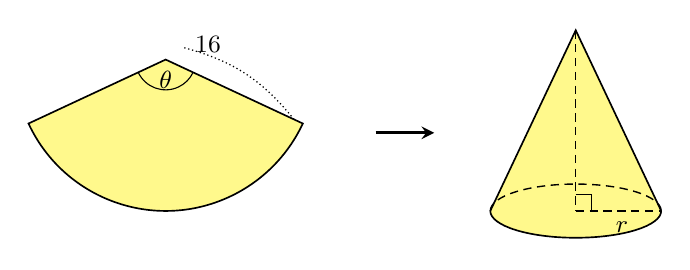
\begin{tikzpicture}[scale=0.62, line width=0.6pt]
  % 부채꼴 종이 — 꼭짓점이 위, 호가 아래
  \fill[yellow!45] (0,0) -- (-155:3.1) arc (-155:-25:3.1) -- cycle;
  \draw (0,0) -- (-155:3.1) arc (-155:-25:3.1) -- cycle;
  \draw[line width=0.4pt] (-155:0.62) arc (-155:-25:0.62);
  \node[font=\small] at (-90:0.42) {$\theta$};
  \draw[densely dotted, line width=0.45pt] (-25:2.9) to[bend right=18] (0.35,0.25);
  \node[anchor=west, font=\small] at (0.4,0.3) {$16$};
  % 화살표
  \draw[->, >=stealth, line width=1pt] (4.3,-1.5) -- (5.5,-1.5);
  % 원뿔
  \begin{scope}[shift={(8.4,-3.1)}]
    \fill[yellow!45] (-1.75,0) arc (180:360:1.75 and 0.55) -- (0,3.7) -- cycle;
    \fill[yellow!45] (-1.75,0) arc (180:0:1.75 and 0.55) -- (0,3.7) -- cycle;
    \draw (-1.75,0) -- (0,3.7) -- (1.75,0);
    \draw (-1.75,0) arc (180:360:1.75 and 0.55);
    \draw[densely dashed, line width=0.5pt] (-1.75,0) arc (180:0:1.75 and 0.55);
    \draw[densely dashed, line width=0.5pt] (0,3.7) -- (0,0);
    \draw[densely dashed, line width=0.5pt] (0,0) -- (1.75,0);
    \draw[line width=0.4pt] (0,0.33) -- (0.33,0.33) -- (0.33,0);
    \node[below=1pt, font=\small] at (0.95,0.04) {$r$};
  \end{scope}
\end{tikzpicture}
